\documentclass[color=usenames,dvipsnames]{beamer}
%\documentclass[color=usenames,dvipsnames,handout]{beamer}

%\usepackage[roman]{../pres1}
\usepackage[sans]{../pres1}
\usepackage{graphicx}
%\usepackage{bm}
%\usepackage{soul}
%\usepackage{color}
\usepackage{pdfpages}
\usepackage{animate}
\usepackage{verbatim}


%\setbeameroption{notes on second screen}
%\renewcommand*\sfdefault{lmss} % cmss, lmss (latin modern), phv (Helvetica) qhv, qag
%\renewcommand*\rmdefault{ptm} %



\begin{document}


% \setlength{\fboxsep}{0pt}


\begin{frame}[plain]
  \begin{center}
    {\LARGE {\bf Applied Population Dynamics} \\
     \Large WILD 5700/7700 \\
     \large January 7, 2019} \par
   \vspace{3mm}
   \rule[0pt]{\textwidth}{.2mm}
   \vspace{3mm}
  \end{center}

%  \vspace{-0.4cm}
  %% \begin{columns}[c]%[c]
  %%   \begin{column}[T]{0.5\textwidth}
  %%     \begin{center}
  %%       \fbox{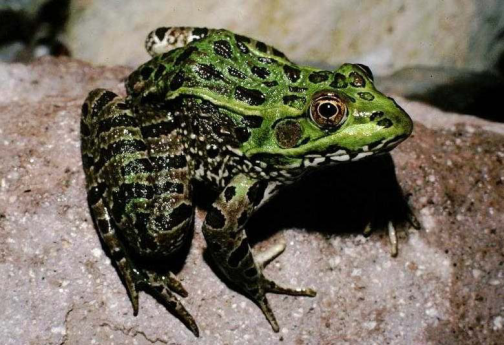
\includegraphics[width=\textwidth]{figs/lich}} \\
  %%       \includegraphics[width=0.9\textwidth]{figs/extinction3}
  %%     \end{center}
  %%     \end{column}
  %%     \begin{column}[T]{0.35\textwidth}
  %%       \begin{center}
  %%         \includegraphics[width=\textwidth]{../../figs/laBear2} \\
  %%         \fbox{\includegraphics[width=\textwidth]{../../figs/bearNF2}}
  %%       \end{center}
  %%     \end{column}
  %%   \end{columns}
  \fbox{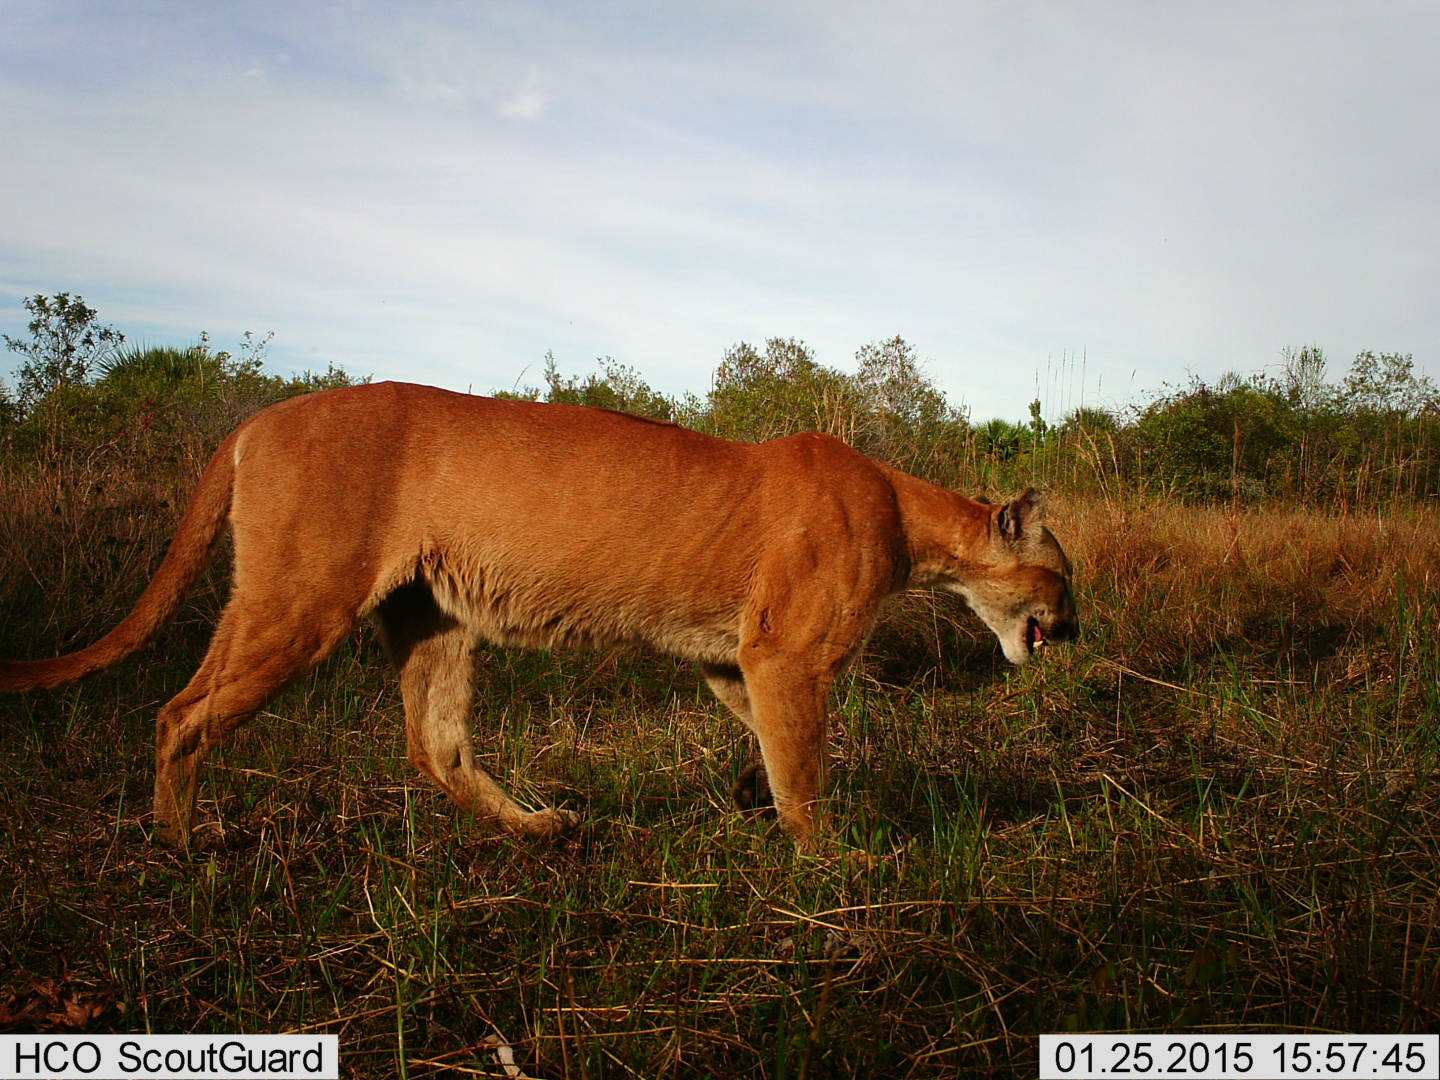
\includegraphics[height=3.9cm,keepaspectratio]{figs/puma1}} \hfill
  \fbox{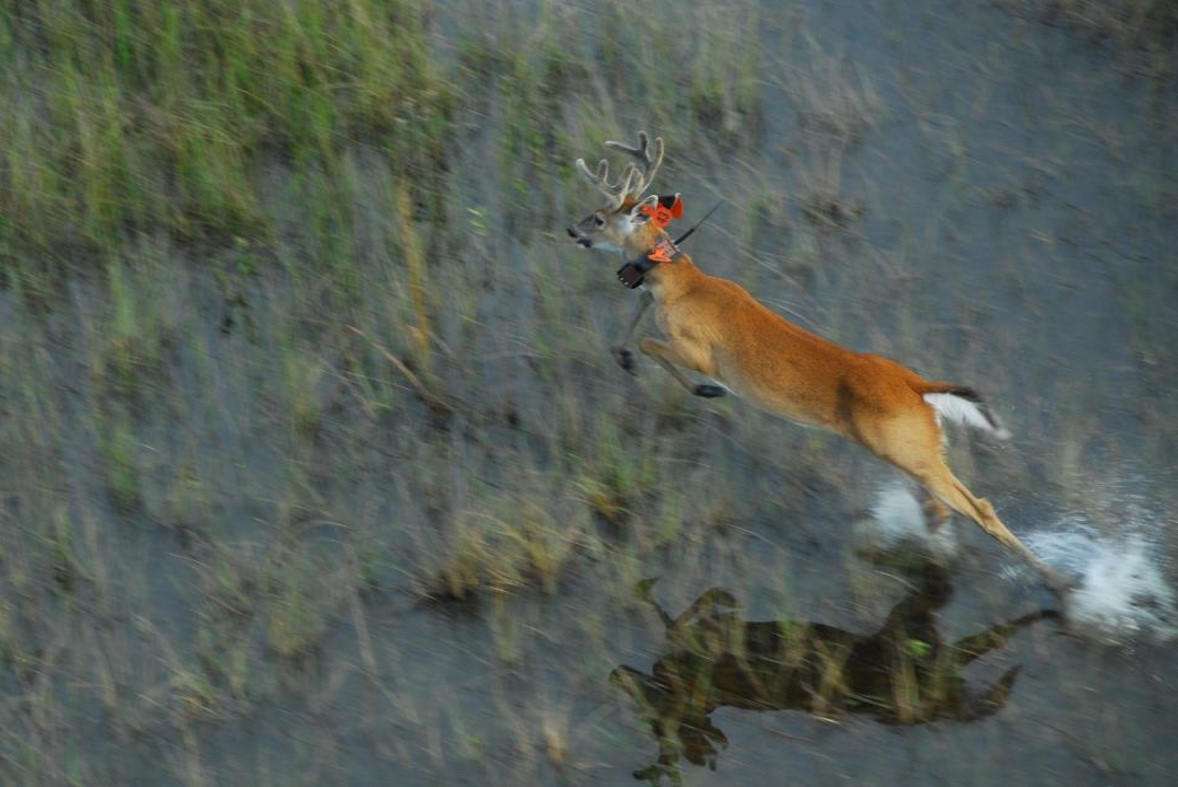
\includegraphics[height=3.9cm,keepaspectratio]{figs/deer_marked_helicopter}}
  \note{Break down the title. Application and theory}
\end{frame}


\note{This topic is imminently important for managers and
  researchers. I didn't have a good class and I regretted it}


\note{Review syllabus}

\note{We will slow down if necessary}

\note{Why do we need so much math? We all wish we could naturalists,
  but we need a balance}

\note{Having said that, We will avoid calculus like the plague. If you
want more calculus, take Population ecology in Odum School}


\note{Teaching philosophy: undergraduates need enough exposure to
  build a solid foundation. Details can only be mastered in practice
  or in grad school.}

\note{Graphs, words, equations}

\note{graduate students should enroll in WILDXXXX if they want the challenge}





%% \begin{frame}
%%   \frametitle{Definitions}
%%   \Large
%%   {\bf Population Dynamics \par}
%%   The study of spatial and temporal variation in population size and
%%   structure \par
%%   \pause
%%   \vspace{1cm}
%%   {\bf Population \par}
%%   A group of individuals of the same species occurring in the same
%%   region during the same time period.
%% \end{frame}





\section{Introduction}






\begin{frame}
\frametitle{Central Questions}
  \Large \centering
  \begin{enumerate}[\bf (1)]
    %   Why do populations vary across space and over time? \par
    \item What causes spatial and temporal variation in population size
    and structure? \par
  % \pause
  % \vspace{0.3cm} {\centering and \dots \par} \vspace{0.3cm} \pause
    \item[]
    \item<2-> How do environmental change and human activities (including
      management actions) affect population dynamics?
  \end{enumerate}
\end{frame}





\begin{frame}
  \frametitle{Learning objectives}
  \large
  {\bf By the end of the semester, you should be able to: \\}
  \vspace{0.3cm}
  \begin{enumerate}[\bf (1)]
    \large
    \item<1-> Develop a population model that
      \begin{itemize}
        \normalsize %\large
        \item Describes variation in demographic parameters over time
        \item Predicts how the population will respond to
          management/conservation actions
      \end{itemize}
    \item[]
    \item<2-> Design a study to collect the data necessary to estimate
      the demographic parameters of the model
    \item[]
    \item<3-> Use software (e.g., {\tt PRESENCE}, {\tt DISTANCE}, {\tt
        MARK}) to estimate parameters from field data
  \end{enumerate}
  \note{If you can do these three things well, you will do well as a
    wildlife ecologist}
\end{frame}







\begin{frame}
  \frametitle{Themes}
  \Large
  \begin{itemize}
    \item[] {\hspace{-0.9cm} \bf Theory}
    \item Population models
    \item[]
    \item[] {\hspace{-0.9cm} \bf Practice (Application)}
    \item Estimation
    \item Harvest management
    \item Small population management
%    \item Population viability analysis
  \end{itemize}
\end{frame}







%% \begin{frame}
%%   \frametitle{Prediction}

%%   We need to predict the future, we do it all the time

%%   Nate Silver

%%   Location of Jupiter
%% \end{frame}






\section{Examples}







\begin{frame}[fragile]
  \frametitle{Example I -- Black-throated blue warbler}
  {\centering \large
    What do these data tell us?
    What don't these data tell us? \par}
\begin{center}
  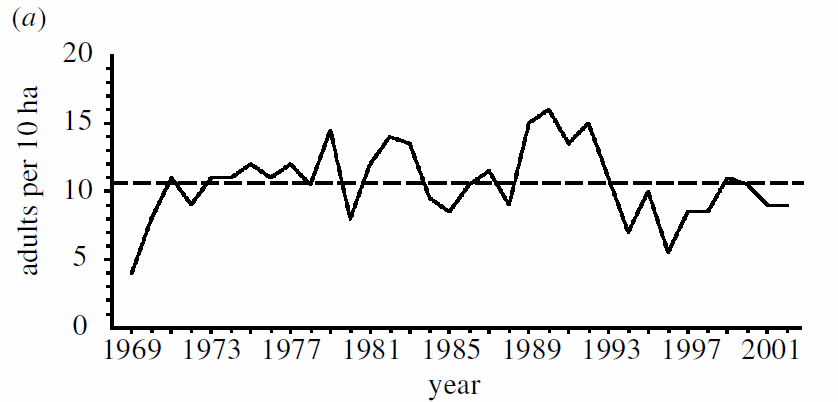
\includegraphics[width=0.9\textwidth]{figs/btbw}\let\thefootnote\relax\footnote{\tiny Rodenhouse et
    al. (2003, Proceedings of the Royle Society)} \\
\end{center}
\hfill 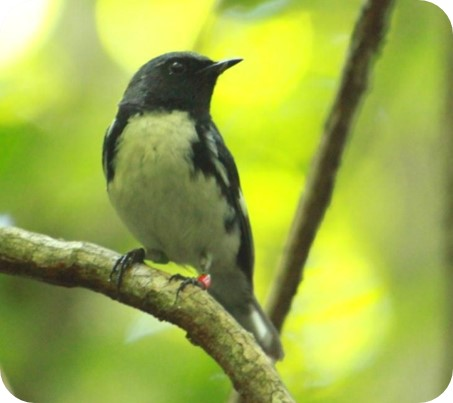
\includegraphics[width=0.2\textwidth]{figs/btbw1}
\end{frame}




\begin{frame}[fragile]
  \frametitle{Example I -- Black-throated blue warbler}
  {\centering \small %\large
    Why are dynamics so different in the southern part of
    the range? \\}
\begin{center}
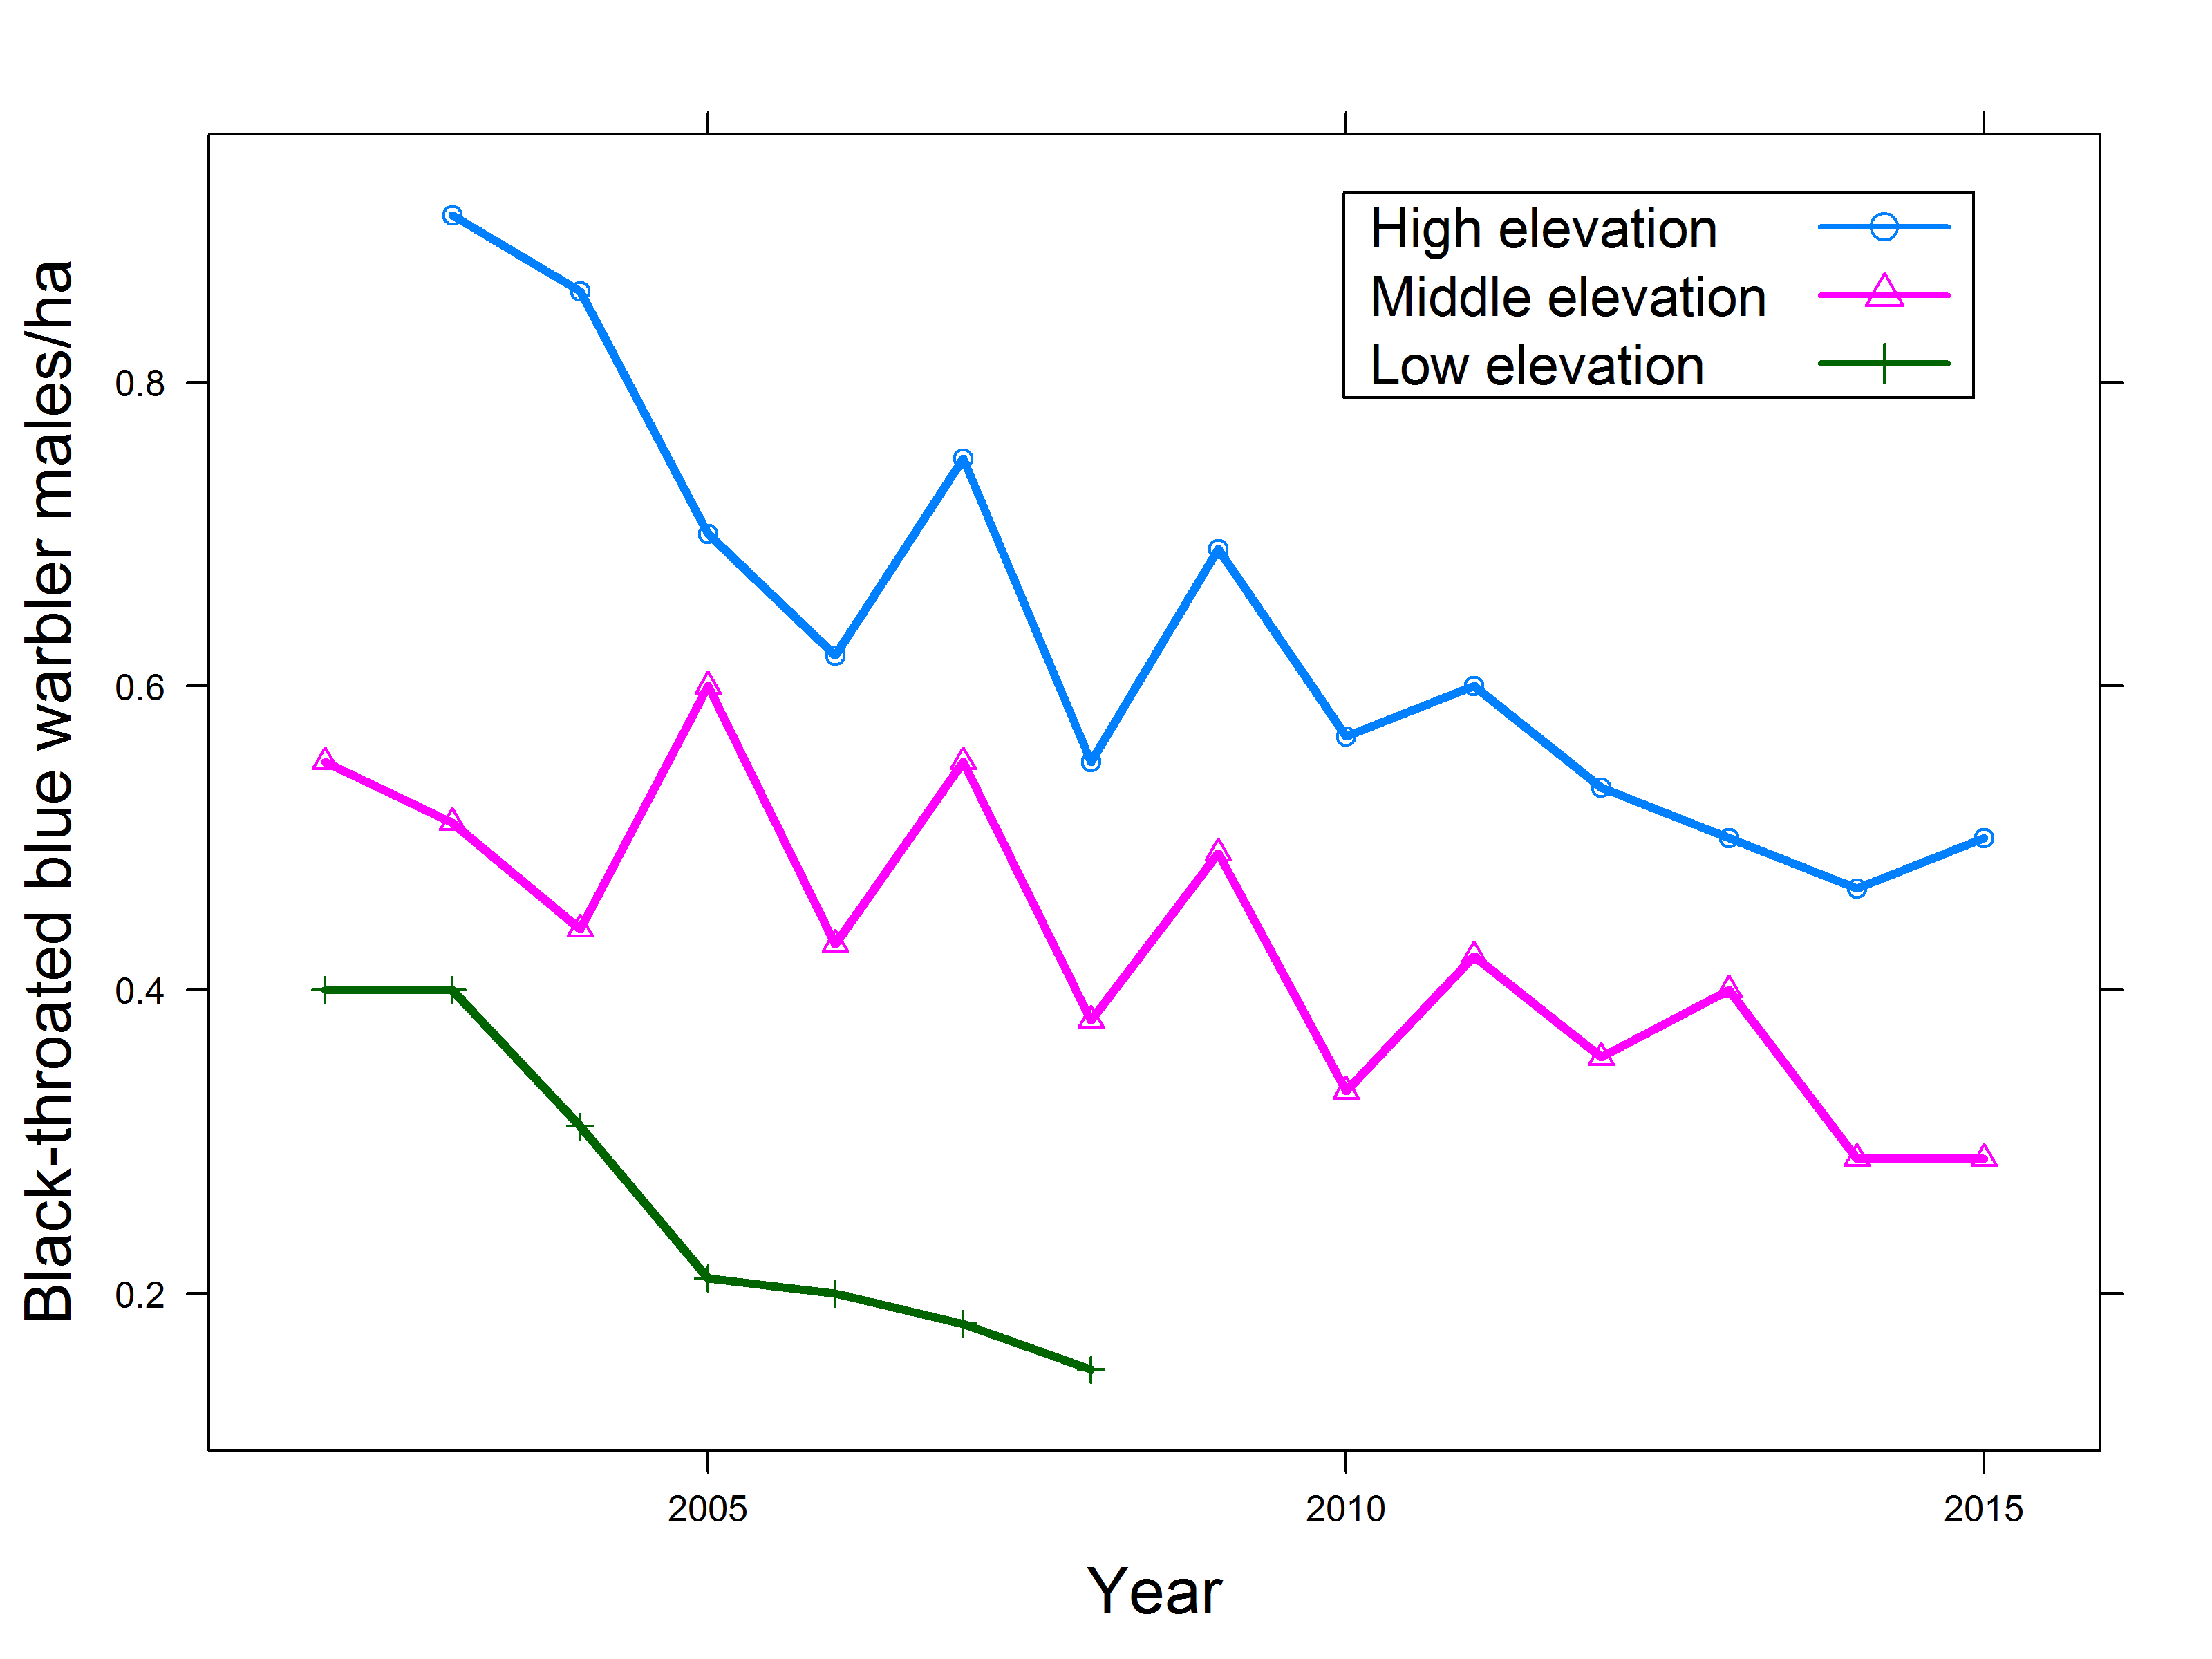
\includegraphics[width=0.8\textwidth]{figs/blue_density3plots}\let\thefootnote\relax\footnote{\tiny
    Data courtesy of Dr. RJ Cooper} 
\end{center}
%\hfill 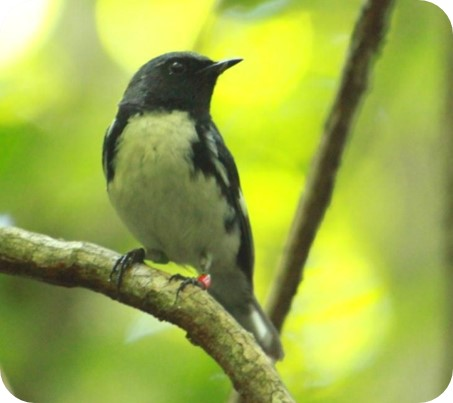
\includegraphics[width=0.2\textwidth]{figs/btbw1}
\end{frame}




\begin{frame}
  \frametitle{Example II -- Louisiana black bear}
  \begin{columns}
    \begin{column}{0.5\textwidth}
      \fbox{\includegraphics[width=\textwidth]{figs/laBear2}}
    \end{column}
    \begin{column}{0.5\textwidth}
      \fbox{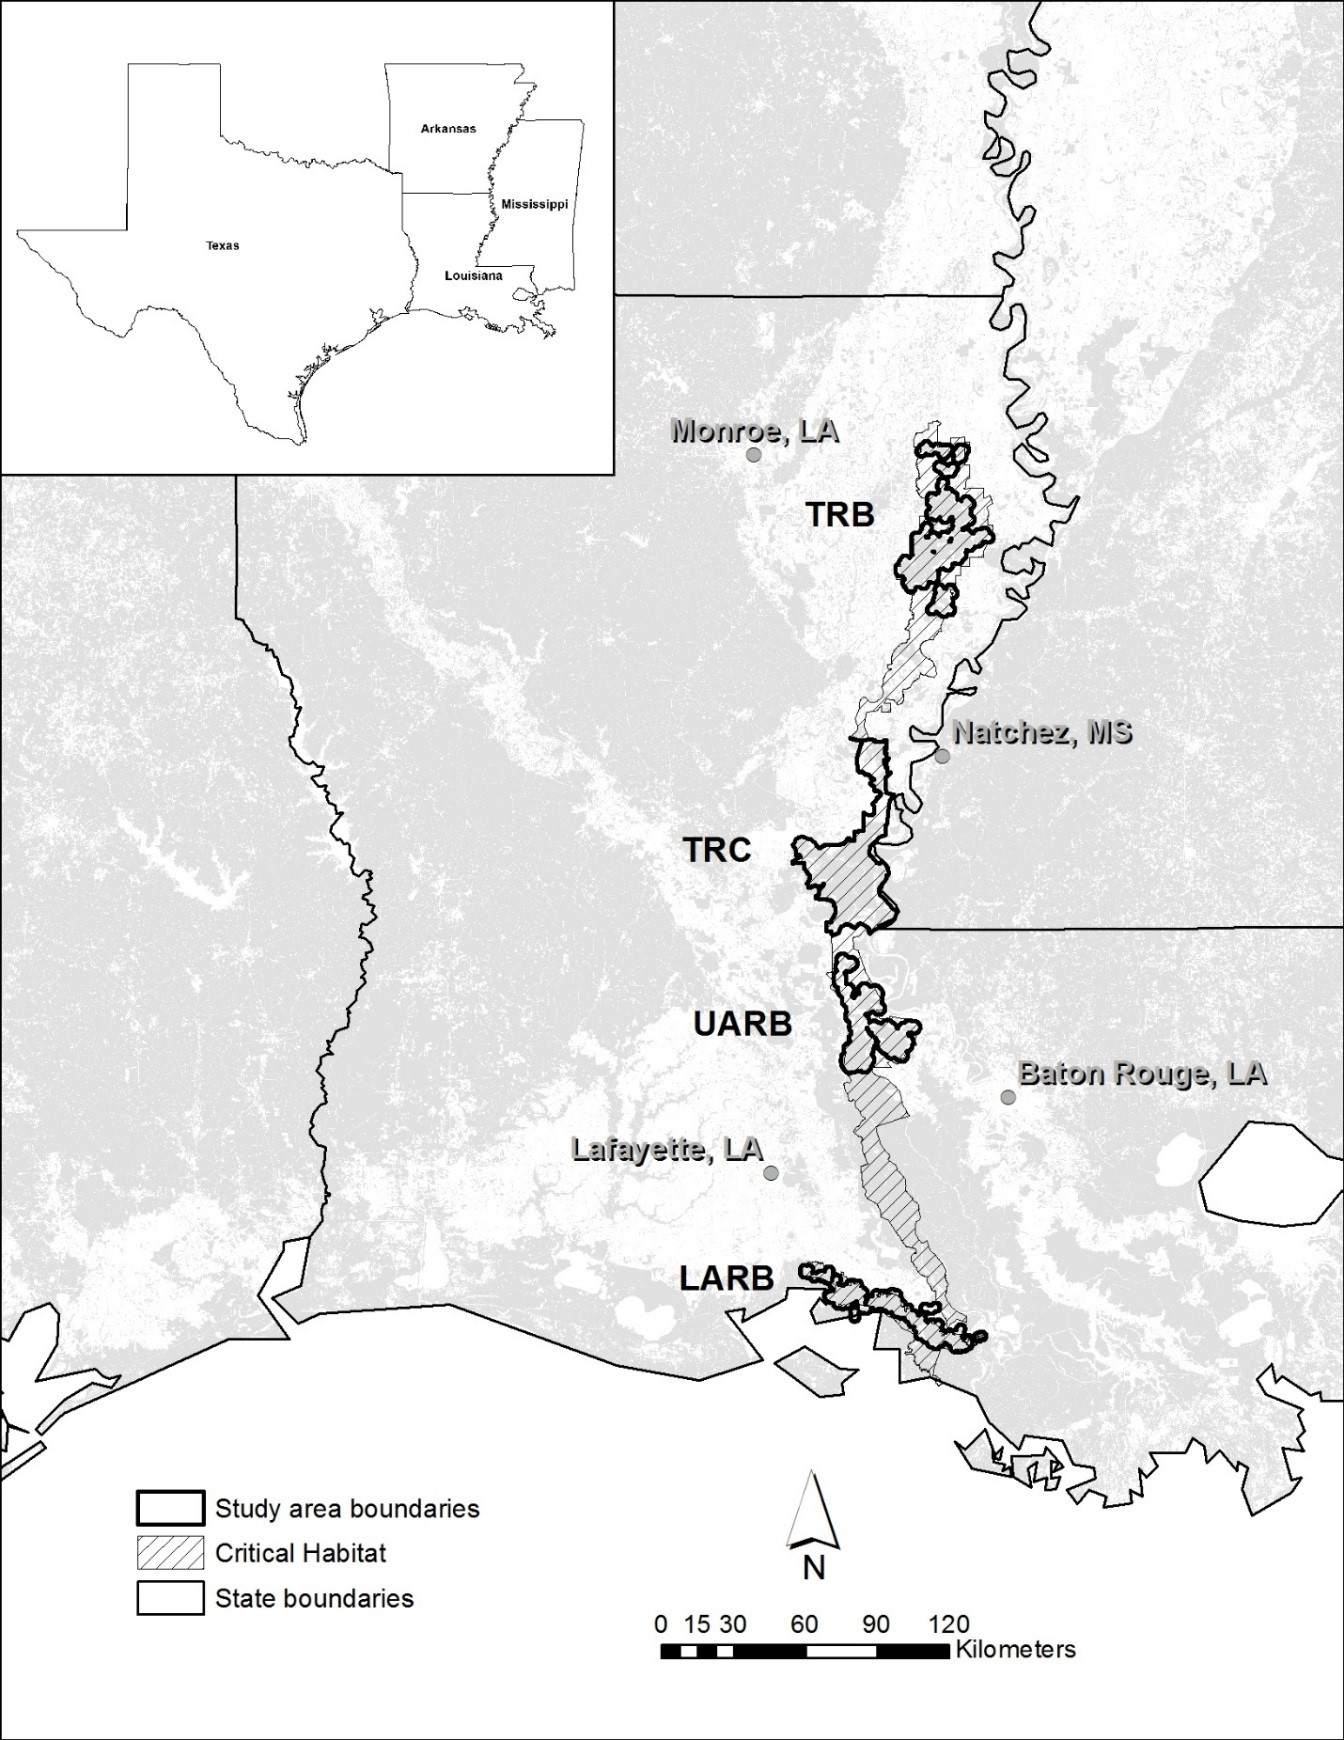
\includegraphics[width=\textwidth]{figs/LA-bear-map}}
    \end{column}
  \end{columns}
\end{frame}


\begin{frame}
  \frametitle{Estimated demographic parameters}
  \begin{center}
    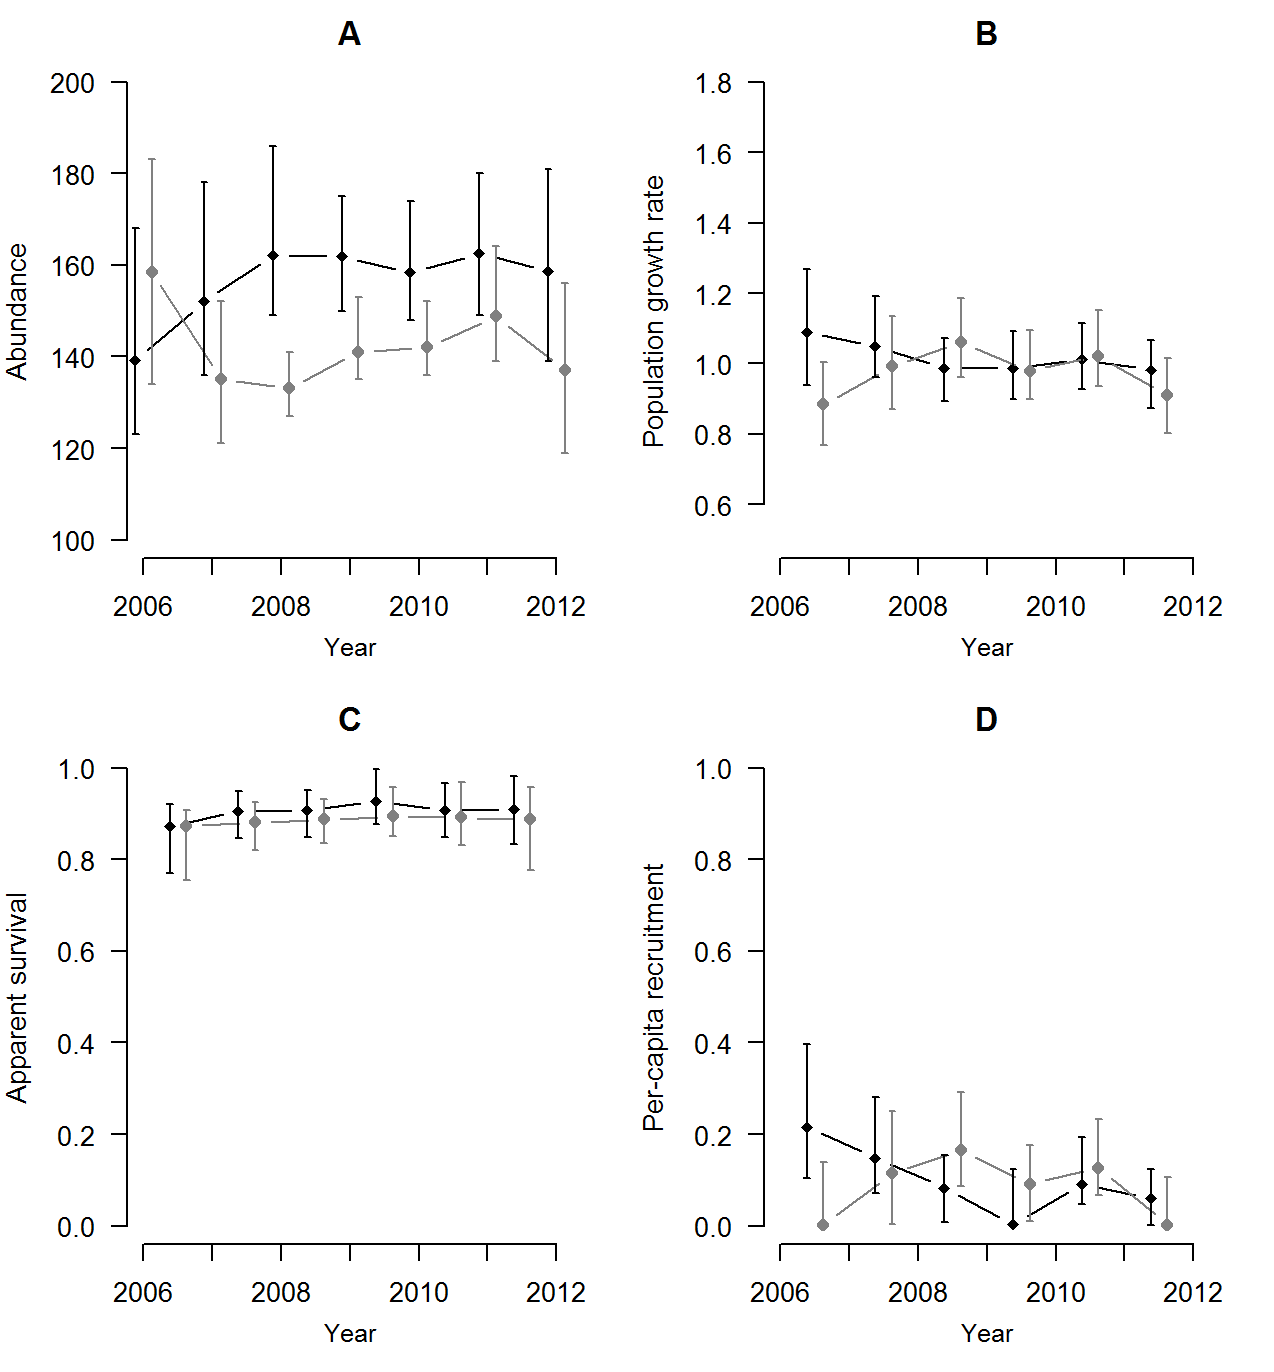
\includegraphics[width=0.7\textwidth]{figs/LA-bear-demographics}
  \end{center}
\end{frame}




\begin{frame}
  \frametitle{Example III -- Chiricahua Leopard Frog}
  \begin{columns}
    \begin{column}{0.5\textwidth}
      \fbox{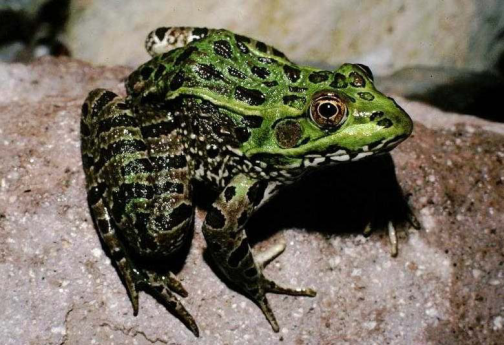
\includegraphics[width=\textwidth]{figs/lich}}
    \end{column}
    \begin{column}{0.5\textwidth}
      \fbox{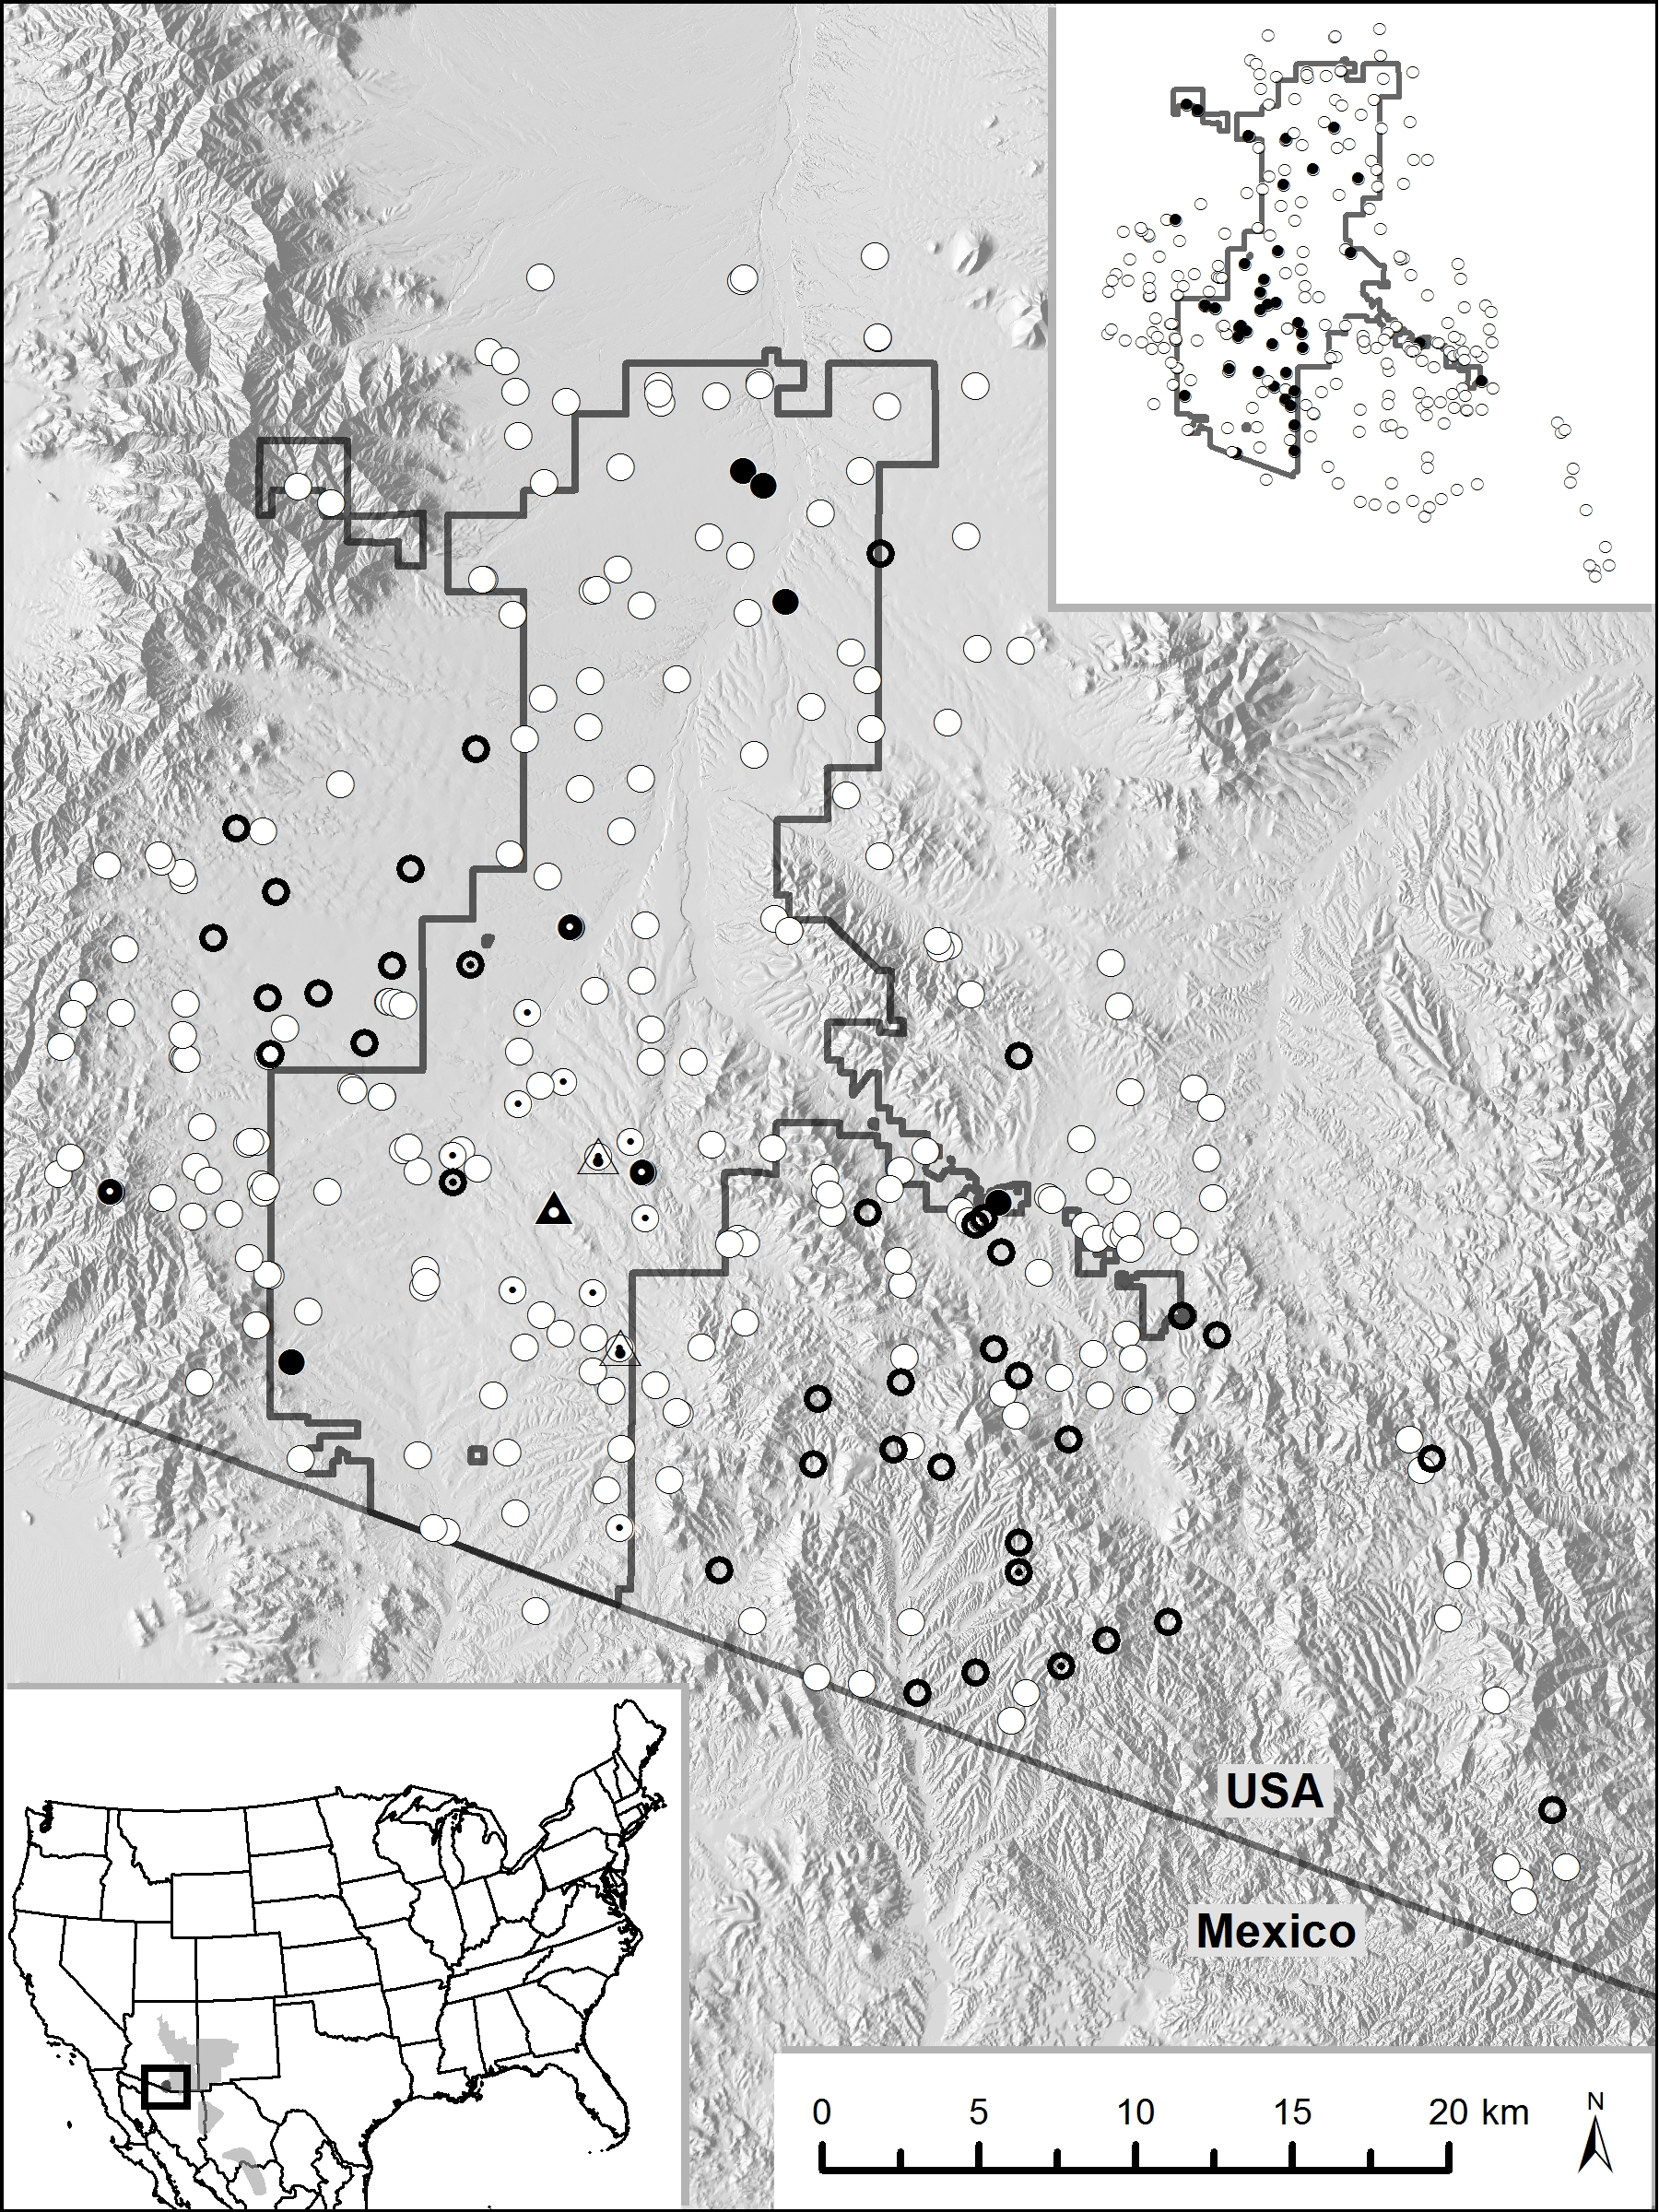
\includegraphics[width=\textwidth]{figs/lich-dist}}
    \end{column}
  \end{columns}
\end{frame}




\begin{frame}
  \frametitle{Recovery Plan}
  \begin{center}
    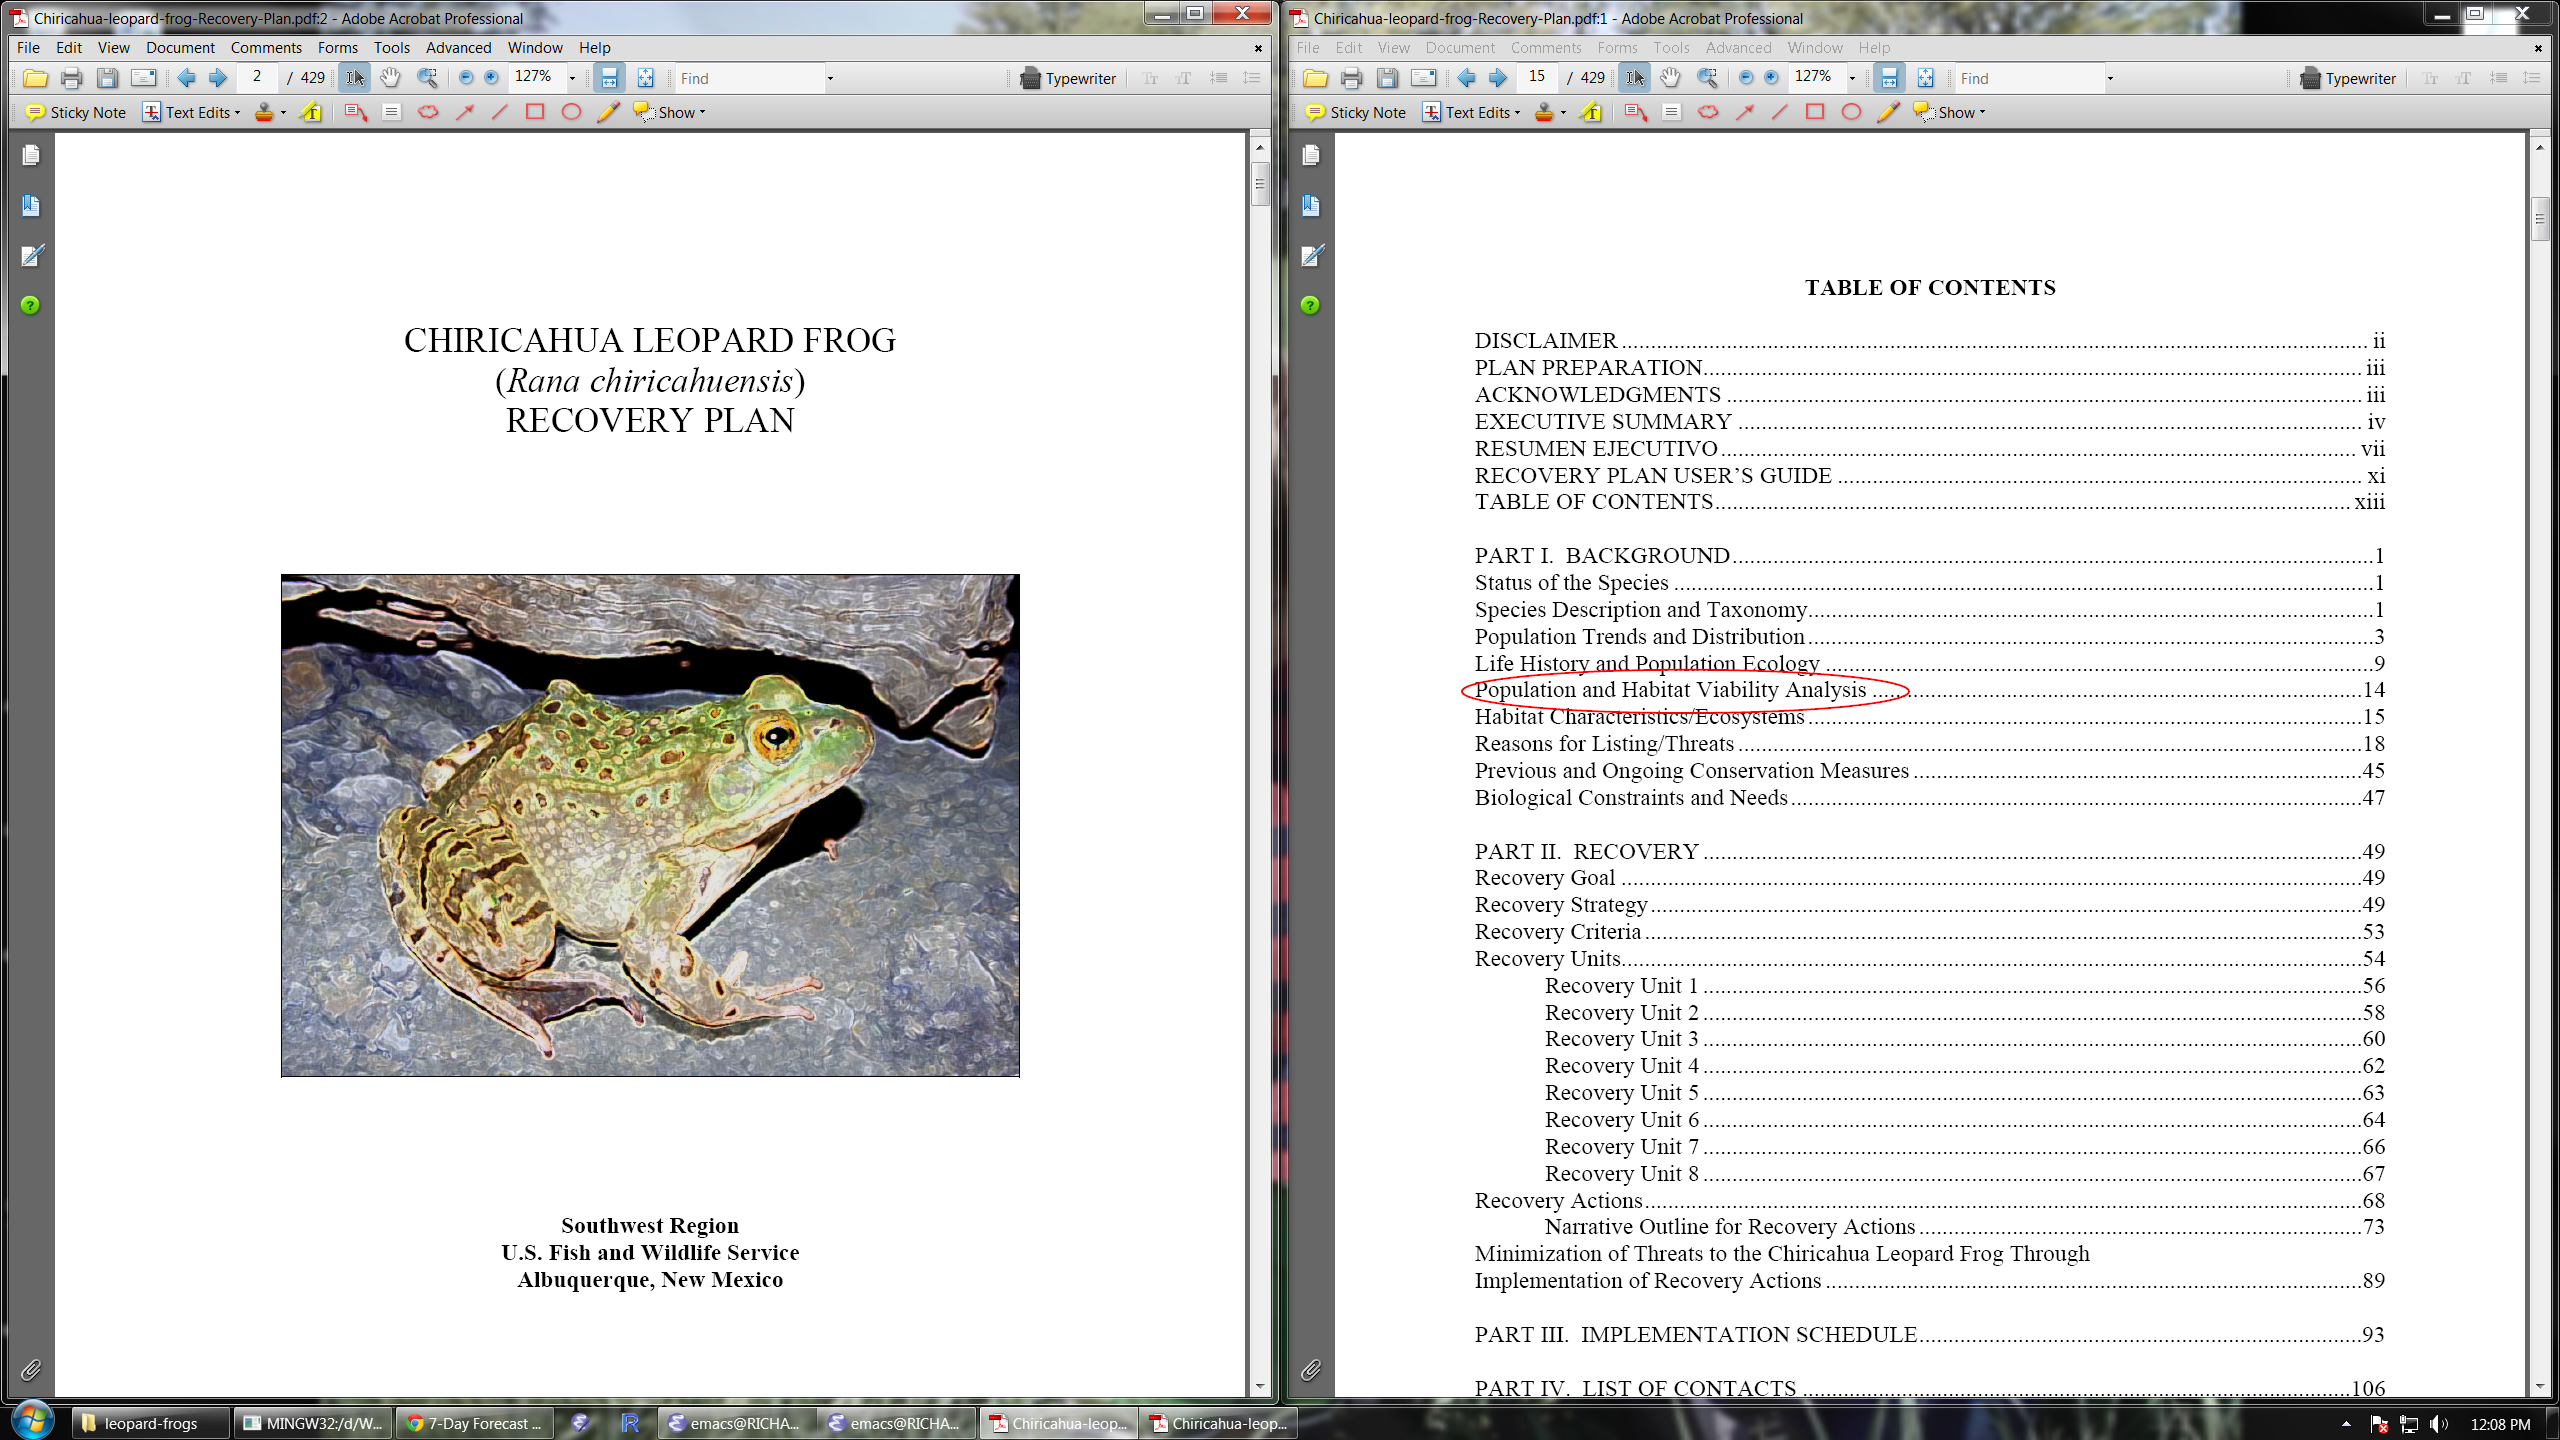
\includegraphics[width=\textwidth]{figs/lich-recovery-plan}
  \end{center}
\end{frame}



\begin{frame}
  \frametitle{Estimated extinction risk}
  \begin{columns}
    \begin{column}{0.6\textwidth}
      \begin{itemize}%[<+->]
      \item<1-> We estimated extinction probability to be $>$2\% by 2100
      \item[]
      \item<2-> What can be done about it?
        \begin{itemize}
        \item<3-> Control predators
        \item<4-> Increase hydroperiod in existing wetlands
        \item<5-> Create new wetlands\dots
        \item<6-> \dots but where?
        \end{itemize}
      \end{itemize}
    \end{column}
    \begin{column}{0.4\textwidth}
      \begin{center}
%        \includegraphics[width=0.4\textwidth]{figs/extinction3}
        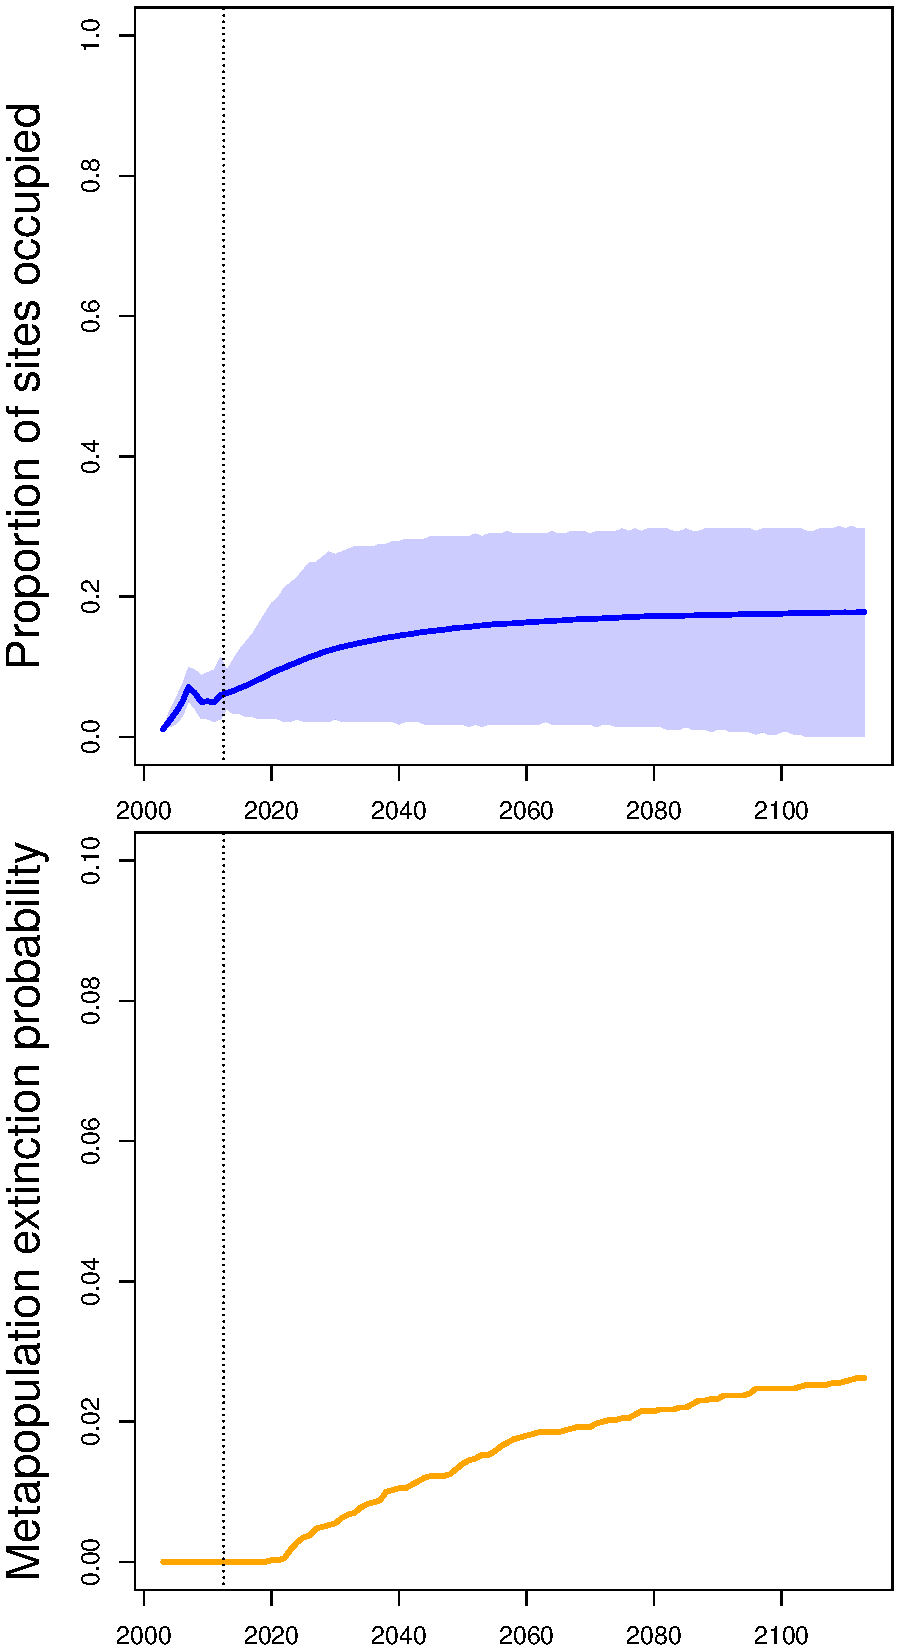
\includegraphics[width=\textwidth]{figs/proj-ext-JAPPL}
      \end{center}
    \end{column}
  \end{columns}
\end{frame}




% \begin{frame}
%   \frametitle{Colonization Probability Maps}
%   \begin{center}
%     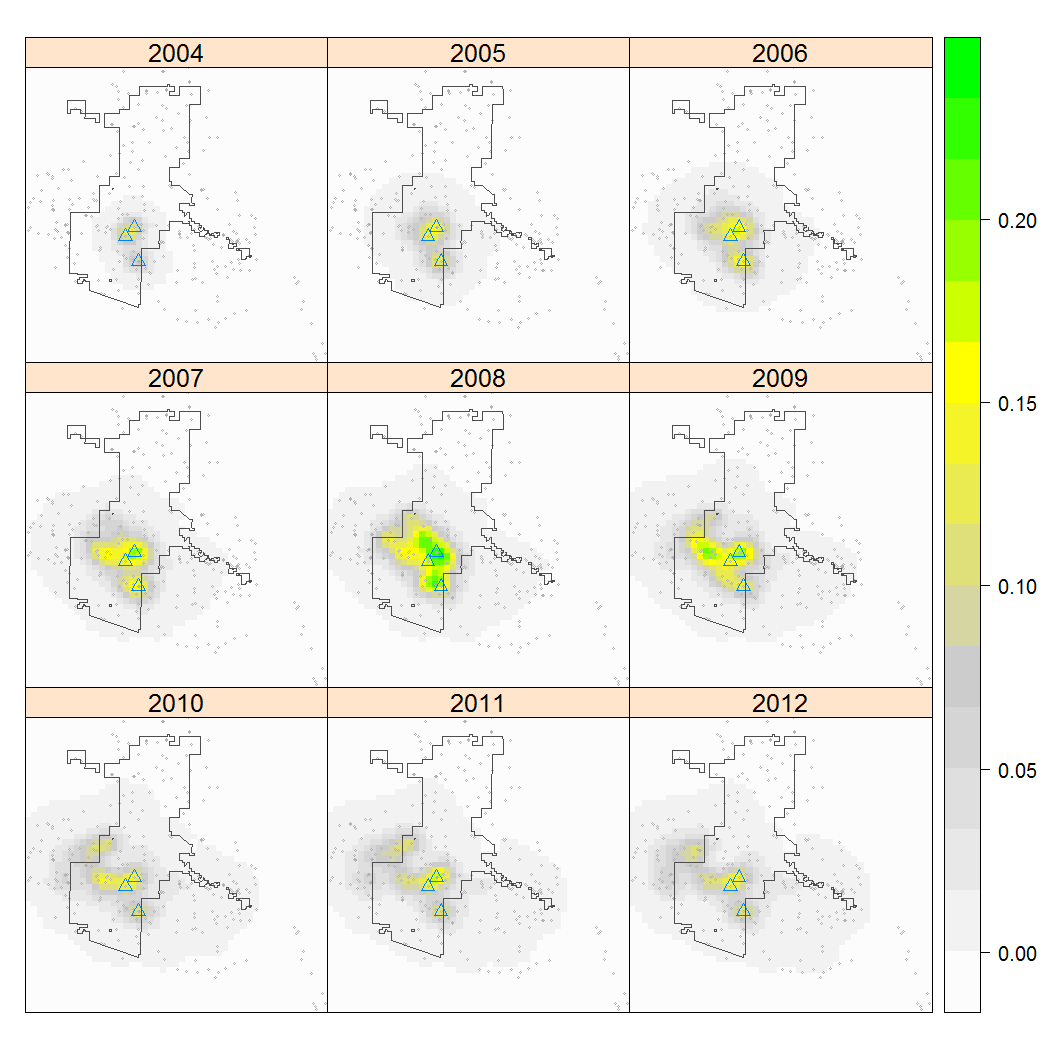
\includegraphics[width=0.7\textwidth]{figs/colMap1-9nohill}
%   \end{center}
% \end{frame}


\begin{frame}
  \frametitle{Colonization Probability Maps}%{Results -- Colonization and connectivity}
  \begin{center}
    \animategraphics[loop,controls,width=0.7\textwidth]{1}{figs/colMap}{2004}{2012} 
    \vfill
  \end{center}
\end{frame}




\begin{frame}
  \frametitle{Example IV -- South Florida Deer Study}
  \large
  {\bf Objectives}
  \begin{enumerate}[\bf (1)]
    \item Understand effects of hydrology, hunting, and predation on
    deer population dynamics 
    \item<1-> Develop a camera trapping study for large-scale
    investigation and monitoring of deer populations
  \end{enumerate}
  \vfill
  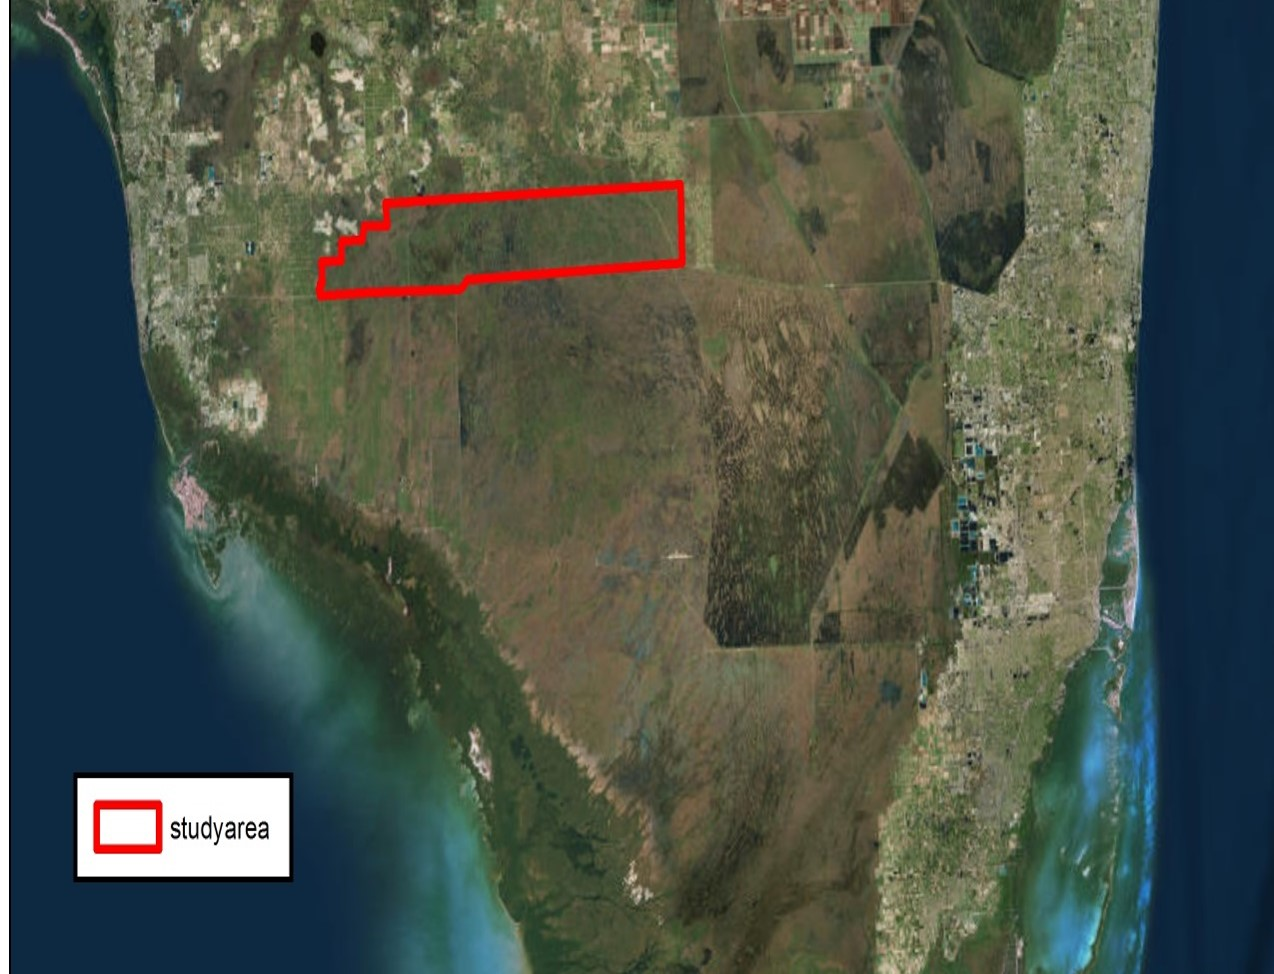
\includegraphics[width=0.49\textwidth,trim = 0mm 8mm 0mm 0mm, clip]{figs/studyArea} \hfill
  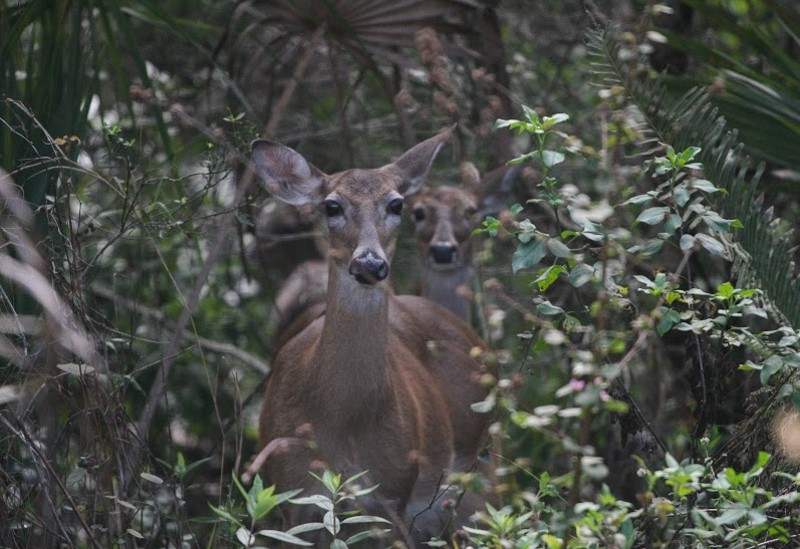
\includegraphics[width=0.49\textwidth]{figs/deer2}
\end{frame}





\begin{frame}
  \frametitle{Camera study}
  \centering
  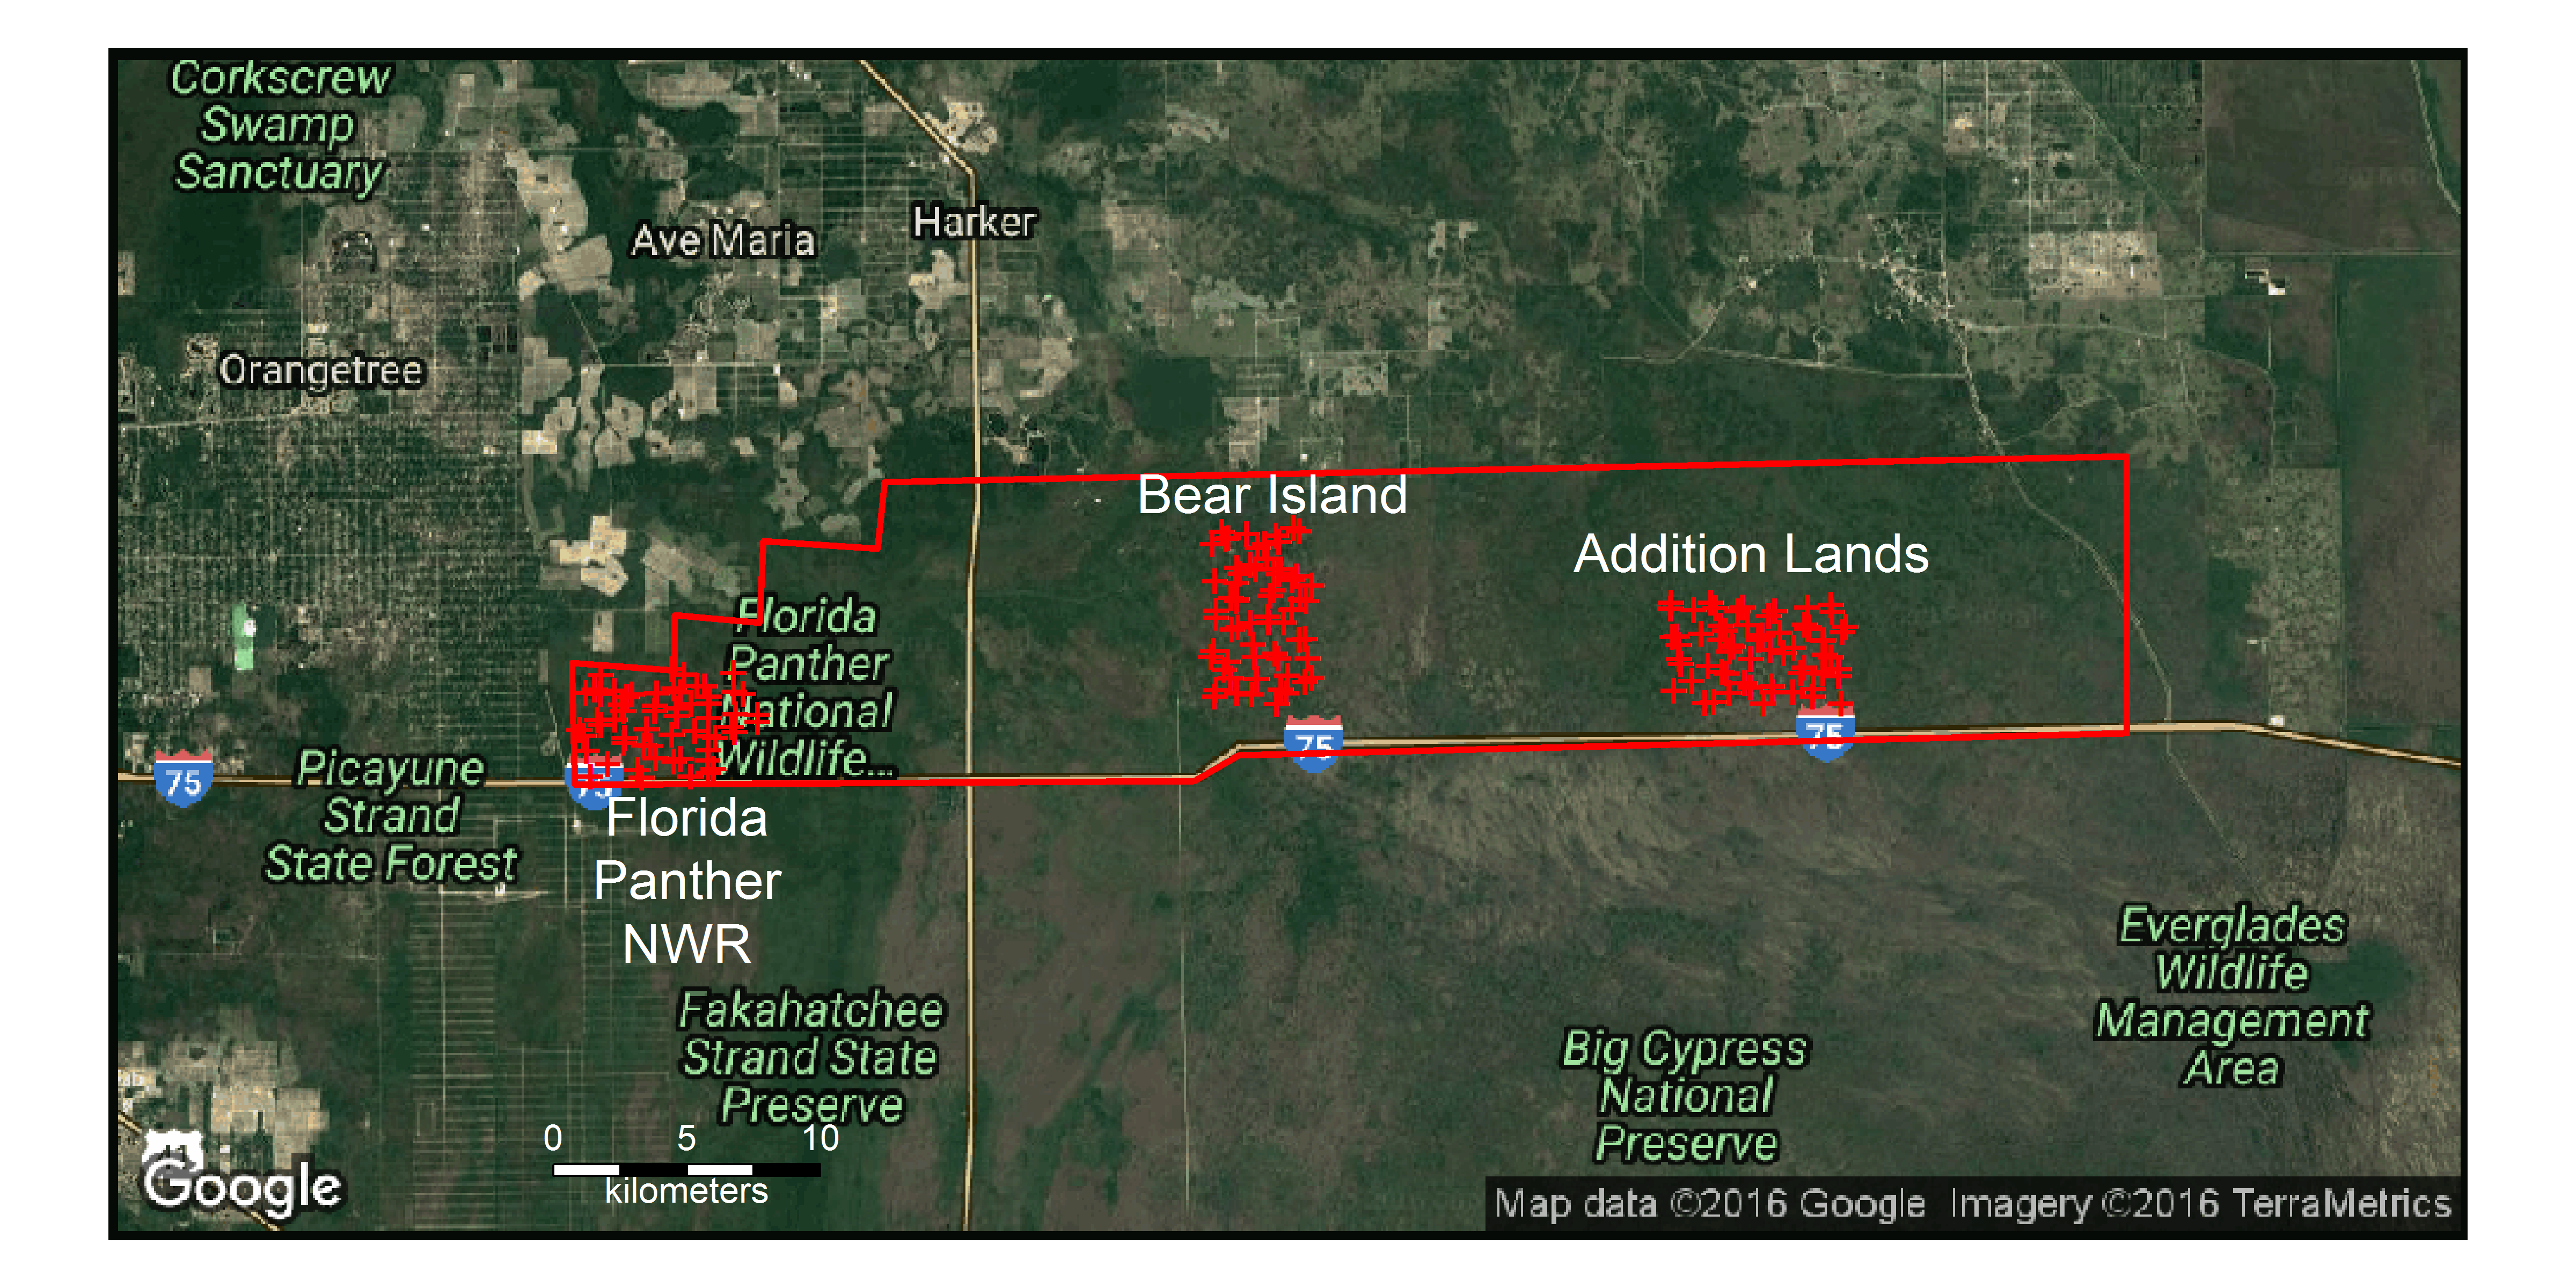
\includegraphics[width=\textwidth]{figs/FL-base-cameras} \\
  \vfill
  \begin{columns}
    \begin{column}{0.05\textwidth}
    \end{column}
    \begin{column}{0.35\textwidth}
      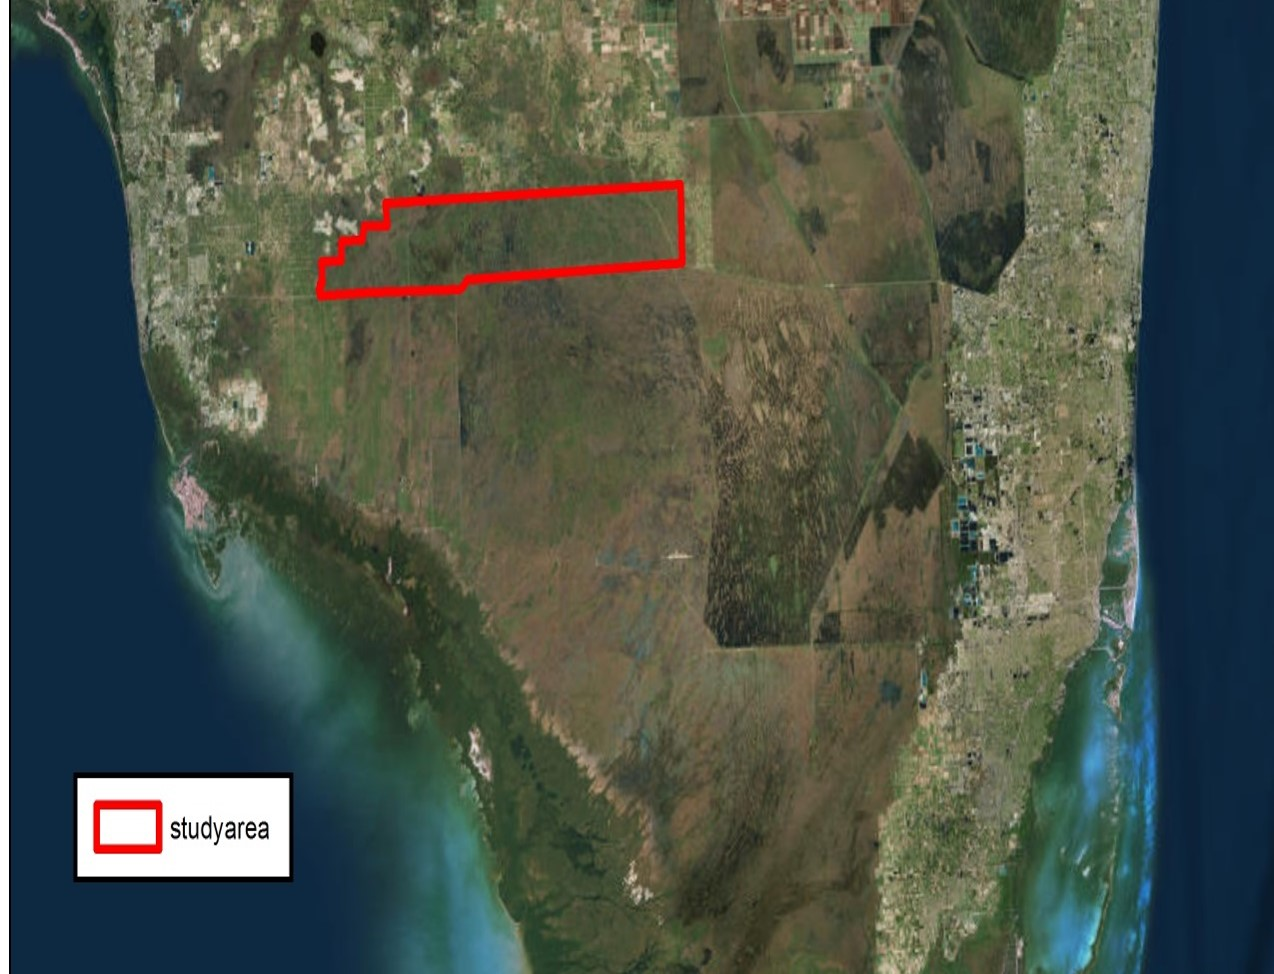
\includegraphics[width=\textwidth,trim = 0mm 8mm 0mm 0mm, clip]{figs/studyArea}
    \end{column}
    \begin{column}{0.6\textwidth}
      \small
      \begin{itemize}
        \item 180 cameras
        \item Operated since January 2015
        \item Spanning hunting and hydrology gradients
      \end{itemize}
    \end{column}
  \end{columns}
\end{frame}



% \begin{frame}
%   \frametitle{Camera data -- temporal view}
%   \only<1>{\includegraphics[width=\textwidth]{figs/All3_camctsInd}} %\\ 
% %  \only<2>{\includegraphics[width=\textwidth]{figs/FP_camctsInd}} 
% \end{frame}



% \begin{frame}
%   \frametitle{Camera data -- spatial view}
% %  \includegraphics[width=\textwidth]{figs/FP_bubble}
%   \includegraphics[width=\textwidth]{../../figs/ALcamdets}
% \end{frame}



\begin{frame}
  \frametitle{Telemetry data}
  \centering
  \bf
  $>$250 deer collared since January 2015 \\
  \begin{columns}
    \column{\dimexpr\paperwidth-10pt}
    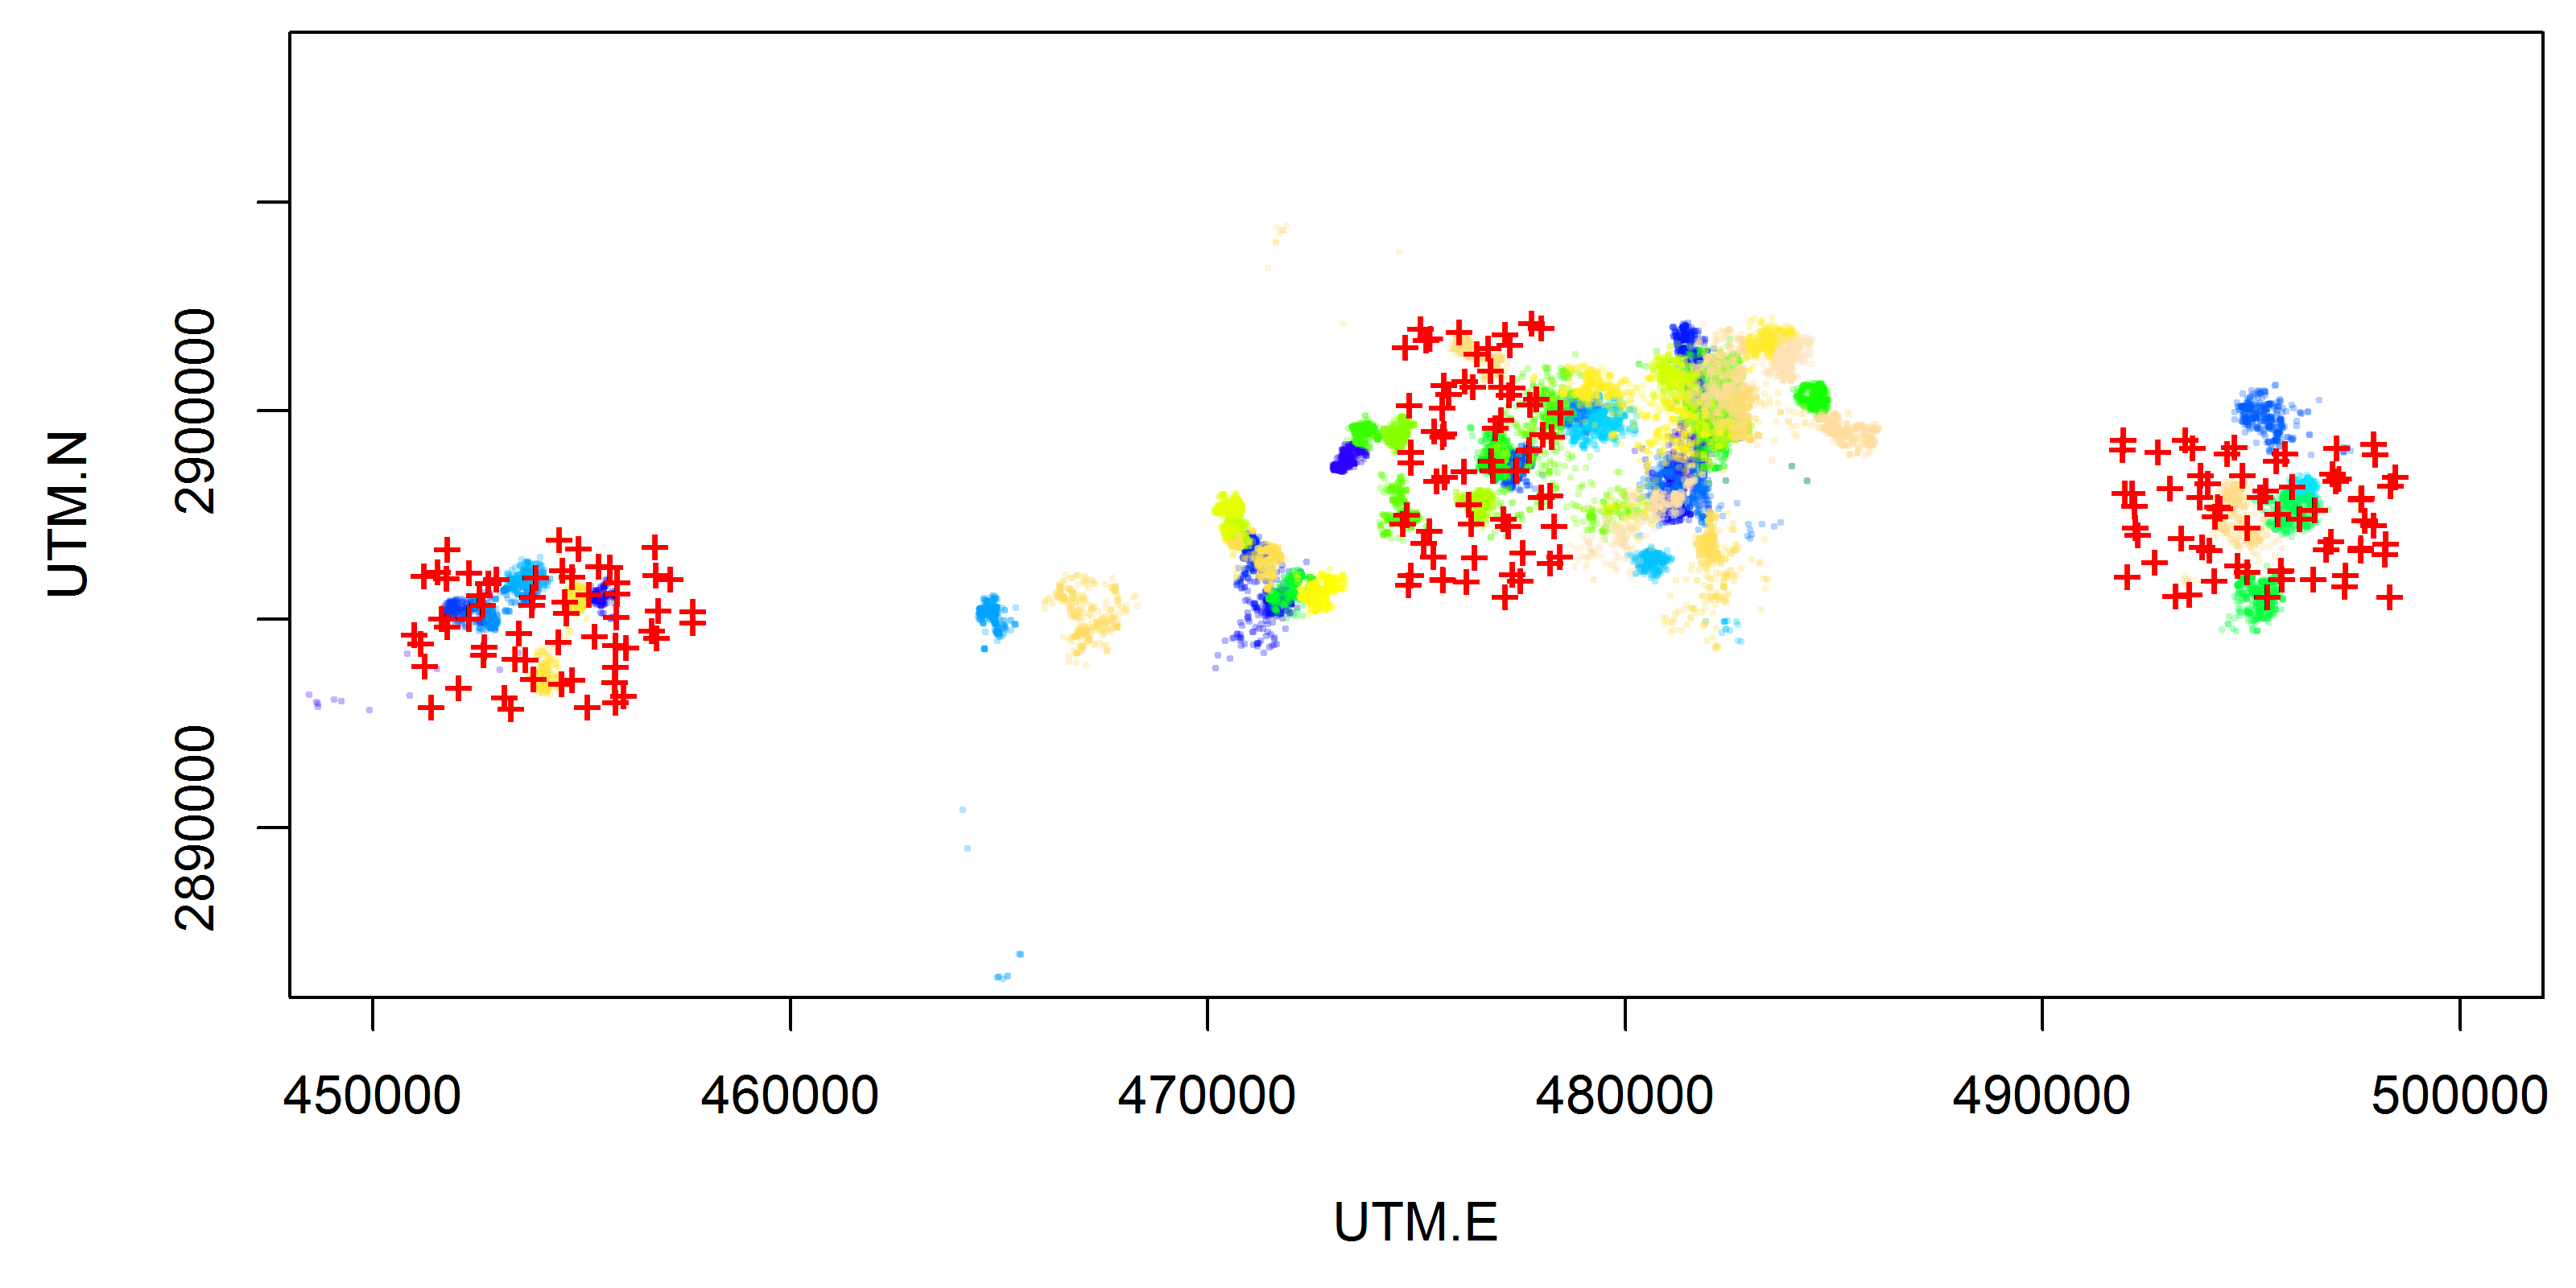
\includegraphics[width=\textwidth]{figs/camTelem}
  \end{columns}
\end{frame}







\section{Syllabus}


\begin{frame}
  \frametitle{Syllabus}
  \begin{columns}%[T]
    \begin{column}{0.5\textwidth}
      \Large %{\bf Syllabus}
      \begin{itemize}
      \item Contact info
      \item Overview
      \item Book
      \item Grading
      \item Academic Honesty
      \item Outline
      \end{itemize}
    \end{column}
    \begin{column}{0.5\textwidth}
%      \includepdf[pages={1},width=\textwidth]{../../syllabus/APD-syllabus.pdf}
      \fbox{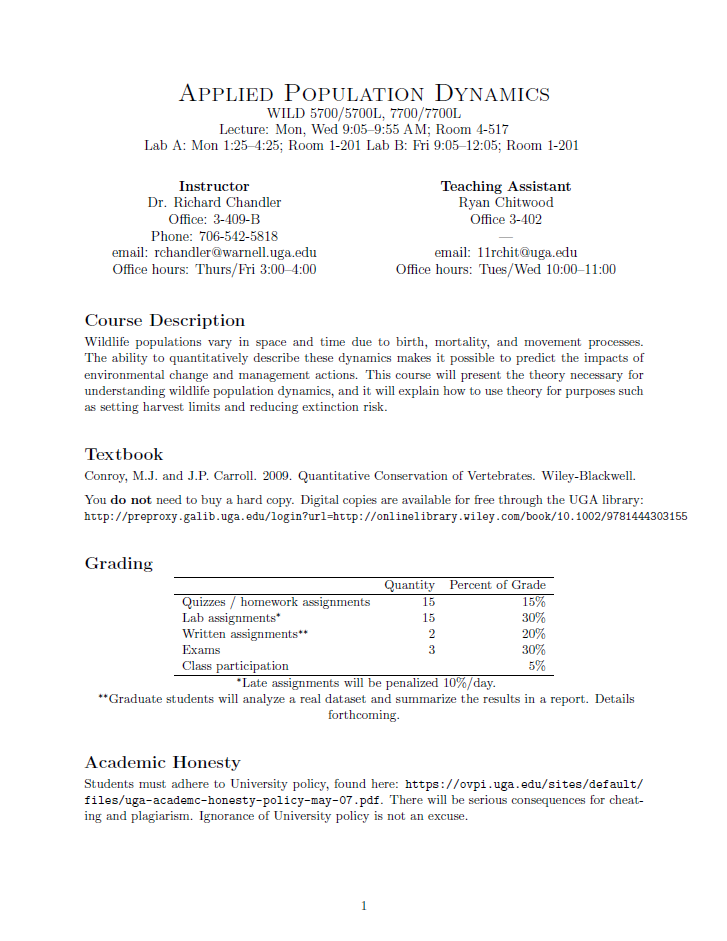
\includegraphics[width=\textwidth]{figs/syllabusP1}}
    \end{column}
  \end{columns}
\end{frame}








\section{Assignment}


\begin{frame}
  \frametitle{Assignment}
  \begin{columns}
    \begin{column}{0.6\textwidth}
      \large
      \begin{enumerate}[\bf (1)]
        \item<1-> Read Chapters 1 and 2 of Conroy and Carroll
        \item[]
        \item<1-> Complete the introductory ``quiz'' found here: \\ \tiny \url{https://goo.gl/forms/OpmugP5lmMrrXTIY2}
      \end{enumerate}
    \end{column}
    \begin{column}{0.4\textwidth}
      \fbox{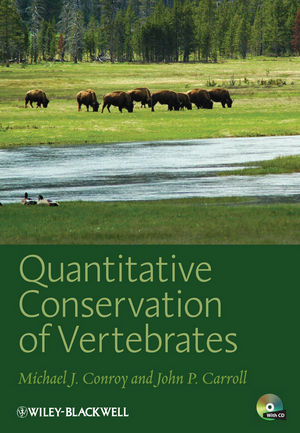
\includegraphics[width=\textwidth]{figs/Conroy_Carroll}}
    \end{column}
  \end{columns}
\end{frame}



\begin{comment}
\begin{frame}
  \frametitle{Survey 1}
%  This will count for 1 point
  \begin{enumerate}[(1)]
    \item What species and/or taxonomic group are you interested in?
    \item How much experience do you have with Excel?
      \begin{itemize}
         \item None
         \item Some
         \item Lots
      \end{itemize}
    \item Are you an undergraduate or graduate student?
    \item What kind of job do you want?
      \begin{itemize}
        \item Academic
        \item Research
        \item Conservation/Management
        \item Other. Describe~\rule{3cm}{0.1mm}
      \end{itemize}
    \item What is the most important skill or concept you hope to
      learn about in this course?
    \item Do you have access a smartphone or a laptop computer that you would
      be willing to bring to class?
  \end{enumerate}
\end{frame}
\end{comment}


\end{document}
